\hypertarget{controller}{%
\section{Controller}\label{controller}}

This project contains different controllers for the PAT system. The
controllers implemented at moment are: Manual, Calibrated, PIDKPA101.

\textbf{Requirements}

\includegraphics{https://img.shields.io/static/v1?label=cpp\&message=11\&color=007bff}

\includegraphics{https://img.shields.io/static/v1?label=cmake\&message=3.16\&color=007bff}

\includegraphics{https://img.shields.io/static/v1?label=git\&message=2.0\&color=007bff}

\includegraphics{https://img.shields.io/static/v1?label=Doxygen\&message=1.8.13\&color=007bff}

\includegraphics{https://img.shields.io/static/v1?label=Sphinx\&message=3.0.2\&color=007bff}

\includegraphics{https://img.shields.io/static/v1?label=OS\&message=Win\&color=28a745\%22}

\hypertarget{generality}{%
\subsection{Generality}\label{generality}}

\hypertarget{import}{%
\subsubsection{Import}\label{import}}

Import as an external library into your project by copy-paste the
following lines in your \texttt{config.json}.

\begin{Shaded}
\begin{Highlighting}[]
\FunctionTok{\{}
  \DataTypeTok{"name"}     \FunctionTok{:} \StringTok{"PATController"}\FunctionTok{,}
  \DataTypeTok{"path"}     \FunctionTok{:} \StringTok{"gitlab.dei.unipd.it/PAT/Controller.git"}\FunctionTok{,}
  \DataTypeTok{"tag"}      \FunctionTok{:} \StringTok{"HEAD"}\FunctionTok{,}
  \DataTypeTok{"available"}\FunctionTok{:} \StringTok{"YES"}\FunctionTok{,}
  \DataTypeTok{"getGui"}   \FunctionTok{:} \StringTok{"YES"}
\FunctionTok{\}}
\end{Highlighting}
\end{Shaded}

\hypertarget{prerequisites}{%
\subsubsection{Prerequisites}\label{prerequisites}}

The following libraries are auto fetched from the gitlab.dei.unipd.it
host (ask the owner of this repo to become a member):

\begin{itemize}
\tightlist
\item
  \href{https://gitlab.dei.unipd.it/PAT/Mirror}{Mirror} 1.0.0
\item
  \href{https://gitlab.dei.unipd.it/PAT/PSD}{PSD} 1.0.0
\item
  \href{https://gitlab.dei.unipd.it/PAT/Camera}{Camera} 1.0.0
\end{itemize}

These other libraries need to be installed manually in your system:

\begin{itemize}
\tightlist
\item
  \href{https://www.qt.io/}{Qt} 5.14.2
\end{itemize}

The library documentation is generated through
\href{http://www.doxygen.nl/download.html}{Doxygen 1.8.13}. Additional
documentation in the \texttt{index} folder is generated through the
\href{https://www.anaconda.com/products/individual}{python3} package
\href{https://www.sphinx-doc.org/en/master/}{Sphinx} using the following
extensions (which you can install through pip3):

\begin{itemize}
\tightlist
\item
  \href{https://pypi.org/project/Sphinx/}{Sphinx 3.0.2}
\item
  \href{https://sphinx-rtd-theme.readthedocs.io/en/stable/}{Sphinx read
  the doc theme} (to use the read the doc theme for html documentation)
\item
  \href{https://pypi.org/project/breathe/}{Breathe} (to use the xml
  output of doxygen)
\item
  \href{https://pypi.org/project/sphinx-markdown-builder/}{Sphinx-markdown-builder}
  (to generate the markdown version for gitlab wiki)
\end{itemize}

\texttt{pip3\ install\ Sphinx\ sphinx\_rtd\_theme\ breathe\ sphinx-markdown-builder}

\hypertarget{usage}{%
\subsection{Usage}\label{usage}}

\hypertarget{pidkpa101}{%
\subsubsection{PIDKPA101}\label{pidkpa101}}

This class offers a set of functions to comunicate with the PID
controller integrated in the KPA101.

First you need to include the header file and use the namespace.

\begin{Shaded}
\begin{Highlighting}[]
\PreprocessorTok{\#include }\ImportTok{\textless{}PAT/Controller/PIDKPA101.h\textgreater{}}
\KeywordTok{using} \KeywordTok{namespace}\NormalTok{ PAT::Controller;}
\end{Highlighting}
\end{Shaded}

When you istantiate the \textbf{PIDKPA101} you must pass a
\textbf{KPA101} istance.

\begin{Shaded}
\begin{Highlighting}[]
\BuiltInTok{std::}\NormalTok{shared\_ptr\textless{}PAT::KPA101\textgreater{} kpa101   = }\BuiltInTok{std::}\NormalTok{make\_shared\textless{}PAT::KPA101\textgreater{}();}
\BuiltInTok{std::}\NormalTok{shared\_ptr\textless{}PAT::Controller::PIDKPA101\textgreater{} pidkpa101 = }\BuiltInTok{std::}\NormalTok{make\_shared\textless{}PAT::Controller::PIDKPA101\textgreater{}(kpa101);}
\end{Highlighting}
\end{Shaded}

You can enable/disable or check if enabled the PIDKPA101 controller
using these functions.

\begin{Shaded}
\begin{Highlighting}[]
\ControlFlowTok{if}\NormalTok{(!pidkpa101{-}\textgreater{}isPIDActive())}
\NormalTok{ pidkpa101{-}\textgreater{}enablePID(}\KeywordTok{true}\NormalTok{);}
\ControlFlowTok{else}
\NormalTok{ pidkpa101{-}\textgreater{}enablePID(}\KeywordTok{false}\NormalTok{);}
\end{Highlighting}
\end{Shaded}

You can set the PID parameters using these functions. PID values are
between 1 and 0.

\begin{Shaded}
\begin{Highlighting}[]
\KeywordTok{auto}\NormalTok{ parameters = pidkpa101{-}\textgreater{}getPIDParameters();}
\NormalTok{parameters.value.proportionalGain = }\DecValTok{1}\NormalTok{;}
\NormalTok{parameters.value.integralGain = }\FloatTok{0.001}\NormalTok{;}
\NormalTok{parameters.value.differentialGain = }\FloatTok{0.01}\NormalTok{;}
\NormalTok{pidkpa101{-}\textgreater{}setPIDParameters(parameters);}
\end{Highlighting}
\end{Shaded}

You can enable/disable the auto open closed loop. If the intensity of
the light is outside the interval \textbf{autoOpenInterval} then the PID
controller is stopped. The intensity value is bounded between 10 and 0.

\begin{Shaded}
\begin{Highlighting}[]
\KeywordTok{auto}\NormalTok{ interval = pidkpa101{-}\textgreater{}getAutoOpenInterval();}
\NormalTok{interval.value.min = }\FloatTok{0.1}\NormalTok{;}
\NormalTok{interval.value.max = }\FloatTok{1.3}\NormalTok{;}
\NormalTok{pidkpa101{-}\textgreater{}setAutoOpenInterval(interval);}
\ControlFlowTok{if}\NormalTok{(!pidkpa101{-}\textgreater{}getAutoOpenCloseLoop())}
\NormalTok{ pidkpa101{-}\textgreater{}setAutoOpenCloseLoop(}\KeywordTok{true}\NormalTok{);}
\end{Highlighting}
\end{Shaded}

The output of the PID controller is multiplied by a feedback constant
that it range between -10 to +10 volts. Using this function you can set
it.

\begin{Shaded}
\begin{Highlighting}[]
\KeywordTok{auto}\NormalTok{ feedback = pidkpa101{-}\textgreater{}getFeedBackGain();}
\NormalTok{gain.value.x = }\DecValTok{10}\NormalTok{;}
\NormalTok{gain.value.y = }\DecValTok{10}\NormalTok{;}
\NormalTok{pidkpa101{-}\textgreater{}setFeedBackGain(feedback);}
\end{Highlighting}
\end{Shaded}

\hypertarget{manual}{%
\subsubsection{Manual}\label{manual}}

Manual is a controller that it allow to move a mirror in the four
directions. It require a \textbf{Mirror} and a \textbf{Centroid}. This
last one is from a \textbf{Frame} inside a \textbf{Camera} or from a
\textbf{PSD}. For semplicity here I provide an example using a
\textbf{IDS} camera and a \textbf{STT254} mirror.

First you need to include the header file and use the namespace.

\begin{Shaded}
\begin{Highlighting}[]
\PreprocessorTok{\#include }\ImportTok{\textless{}PAT/Controller/Manual.h\textgreater{}}
\PreprocessorTok{\#include }\ImportTok{\textless{}PAT/Mirror/STT254.h\textgreater{}}
\PreprocessorTok{\#include }\ImportTok{\textless{}PAT/Camera/IDS.h\textgreater{}}
\KeywordTok{using} \KeywordTok{namespace}\NormalTok{ PAT::Controller;}
\KeywordTok{using} \KeywordTok{namespace}\NormalTok{ PAT::Camera;}
\KeywordTok{using} \KeywordTok{namespace}\NormalTok{ PAT::Mirror;}
\end{Highlighting}
\end{Shaded}

When you istantiate the \textbf{Manual} you must pass a \textbf{Mirror}
and a \textbf{Centroid} istances.

\begin{Shaded}
\begin{Highlighting}[]
\BuiltInTok{std::}\NormalTok{shared\_ptr\textless{}Camera\textgreater{} camera      = }\BuiltInTok{std::}\NormalTok{make\_shared\textless{}IDS\textgreater{}();}
\BuiltInTok{std::}\NormalTok{shared\_ptr\textless{}PAT::KPA101\textgreater{} kpa101 = }\BuiltInTok{std::}\NormalTok{make\_shared\textless{}PAT::KPA101\textgreater{}();}
\BuiltInTok{std::}\NormalTok{shared\_ptr\textless{}Mirror\textgreater{} mirror      = }\BuiltInTok{std::}\NormalTok{make\_shared\textless{}STT254\textgreater{}(kpa101);}
\BuiltInTok{std::}\NormalTok{shared\_ptr\textless{}Manual\textgreater{} manual      = }\BuiltInTok{std::}\NormalTok{make\_shared\textless{}Manual\textgreater{}(mirror, camera{-}\textgreater{}getFrame(){-}\textgreater{}getCentroid());}
\end{Highlighting}
\end{Shaded}

To move in one of the four directions you can use this code.

\begin{Shaded}
\begin{Highlighting}[]
\NormalTok{manual{-}\textgreater{}move(Direction::up);}
\NormalTok{manual{-}\textgreater{}move(Direction::down);}
\NormalTok{manual{-}\textgreater{}move(Direction::left);}
\NormalTok{manual{-}\textgreater{}move(Direction::right);}
\end{Highlighting}
\end{Shaded}

To choose how much move you need to set times (milliseconds) and
voltages (volts) in the four directions. You can also control the
current values.

\begin{Shaded}
\begin{Highlighting}[]
\ControlFlowTok{if}\NormalTok{(manual{-}\textgreater{}getManualVoltage(Direction::up) \textgreater{} }\DecValTok{100}\NormalTok{)}
\NormalTok{  manual{-}\textgreater{}setManualVoltage(}\DecValTok{1}\NormalTok{, Direction::up);}
\ControlFlowTok{if}\NormalTok{(manual{-}\textgreater{}getManualTime(Direction::up) \textgreater{} }\DecValTok{100}\NormalTok{)}
\NormalTok{  manual{-}\textgreater{}setManualTime(}\DecValTok{1}\NormalTok{, Direction::down);}
\end{Highlighting}
\end{Shaded}

You can also invert or check the movement directions in the two axes.
You can also swap the two axes.

\begin{Shaded}
\begin{Highlighting}[]
\ControlFlowTok{if}\NormalTok{(!manual{-}\textgreater{}getFlippedX())}
\NormalTok{ manual{-}\textgreater{}setFlippedX(}\KeywordTok{true}\NormalTok{);}
\ControlFlowTok{else}
\NormalTok{ manual{-}\textgreater{}setFlippedX(}\KeywordTok{false}\NormalTok{);}

\ControlFlowTok{if}\NormalTok{(!manual{-}\textgreater{}getFlippedY())}
\NormalTok{ manual{-}\textgreater{}setFlippedY(}\KeywordTok{true}\NormalTok{);}
\ControlFlowTok{else}
\NormalTok{ manual{-}\textgreater{}setFlippedY(}\KeywordTok{false}\NormalTok{);}

\ControlFlowTok{if}\NormalTok{(!manual{-}\textgreater{}getSwappedXY())}
\NormalTok{ manual{-}\textgreater{}setSwappedXY(}\KeywordTok{true}\NormalTok{);}
\ControlFlowTok{else}
\NormalTok{ manual{-}\textgreater{}setSwappedXY(}\KeywordTok{false}\NormalTok{);}
\end{Highlighting}
\end{Shaded}

\hypertarget{manualwidget}{%
\subsubsection{ManualWidget}\label{manualwidget}}

The \textbf{ManualWidget} class is a widget for the Manual controller.
Here I present the an example consistent with the Manual one. The
include code is the following.

\begin{Shaded}
\begin{Highlighting}[]
\PreprocessorTok{\#include }\ImportTok{\textless{}QApplication\textgreater{}}
\PreprocessorTok{\#include }\ImportTok{\textless{}PAT/Controller/gui/ManualWidget.h\textgreater{}}
\PreprocessorTok{\#include }\ImportTok{\textless{}PAT/Mirror/STT254.h\textgreater{}}
\PreprocessorTok{\#include }\ImportTok{\textless{}memory\textgreater{}}
\PreprocessorTok{\#include }\ImportTok{\textless{}PAT/Camera/IDS.h\textgreater{}}
\KeywordTok{using} \KeywordTok{namespace}\NormalTok{ PAT::Controller;}
\KeywordTok{using} \KeywordTok{namespace}\NormalTok{ PAT::Camera;}
\KeywordTok{using} \KeywordTok{namespace}\NormalTok{ PAT::Mirror;}
\end{Highlighting}
\end{Shaded}

This is a simple \textbf{main} example.

\begin{Shaded}
\begin{Highlighting}[]
\DataTypeTok{int}\NormalTok{ main(}\DataTypeTok{int}\NormalTok{ argc, }\DataTypeTok{char}\NormalTok{ *argv[]) \{}
  \ExtensionTok{QApplication}\NormalTok{ a(argc, argv);}
\NormalTok{  ManualWidget manualWidget;}
  \BuiltInTok{std::}\NormalTok{shared\_ptr\textless{}Camera\textgreater{} camera      = }\BuiltInTok{std::}\NormalTok{make\_shared\textless{}IDS\textgreater{}();}
  \BuiltInTok{std::}\NormalTok{shared\_ptr\textless{}PAT::KPA101\textgreater{} kpa101 = }\BuiltInTok{std::}\NormalTok{make\_shared\textless{}PAT::KPA101\textgreater{}();}
  \BuiltInTok{std::}\NormalTok{shared\_ptr\textless{}Mirror\textgreater{} mirror      = }\BuiltInTok{std::}\NormalTok{make\_shared\textless{}STT254\textgreater{}(kpa101);}
  \BuiltInTok{std::}\NormalTok{shared\_ptr\textless{}Manual\textgreater{} manual      = }\BuiltInTok{std::}\NormalTok{make\_shared\textless{}Manual\textgreater{}(mirror, camera{-}\textgreater{}getFrame(){-}\textgreater{}getCentroid());}
\NormalTok{  manualWidget.setController(manual);}
\NormalTok{  manualWidget.show();}
\NormalTok{  camera{-}\textgreater{}start();}
  \ControlFlowTok{return}\NormalTok{ a.exec();}
\NormalTok{\}}
\end{Highlighting}
\end{Shaded}

If you want instead integrate the widget into another GUI (layout) you
can use this code.

\begin{Shaded}
\begin{Highlighting}[]
\ExtensionTok{QWidget}\NormalTok{ *window                     = }\KeywordTok{new} \ExtensionTok{QWidget}\NormalTok{();}
\ExtensionTok{QVBoxLayout}\NormalTok{ *mainLayout             = }\KeywordTok{new} \ExtensionTok{QVBoxLayout}\NormalTok{();}
\NormalTok{ManualWidget *manualWidget          = }\KeywordTok{new}\NormalTok{ ManualWidget();}

\BuiltInTok{std::}\NormalTok{shared\_ptr\textless{}Camera\textgreater{} camera      = }\BuiltInTok{std::}\NormalTok{make\_shared\textless{}IDS\textgreater{}();}
\BuiltInTok{std::}\NormalTok{shared\_ptr\textless{}PAT::KPA101\textgreater{} kpa101 = }\BuiltInTok{std::}\NormalTok{make\_shared\textless{}PAT::KPA101\textgreater{}();}
\BuiltInTok{std::}\NormalTok{shared\_ptr\textless{}Mirror\textgreater{} mirror      = }\BuiltInTok{std::}\NormalTok{make\_shared\textless{}STT254\textgreater{}(kpa101);}
\BuiltInTok{std::}\NormalTok{shared\_ptr\textless{}Manual\textgreater{} manual      = }\BuiltInTok{std::}\NormalTok{make\_shared\textless{}Manual\textgreater{}(mirror, camera{-}\textgreater{}getFrame(){-}\textgreater{}getCentroid());}

\NormalTok{manualWidget{-}\textgreater{}setPSD(manual);}
\NormalTok{mainLayout{-}\textgreater{}addWidget((}\ExtensionTok{QWidget}\NormalTok{ *)manualWidget);}
\NormalTok{window{-}\textgreater{}setLayout(mainLayout);}
\NormalTok{window{-}\textgreater{}show();}
\end{Highlighting}
\end{Shaded}

There are also these three signal functions that they are used to
propagate the click of their respective buttons in other controllers.

\begin{Shaded}
\begin{Highlighting}[]
\DataTypeTok{void}\NormalTok{ chkFlipXchanged(}\DataTypeTok{int}\NormalTok{ arg1);}
\DataTypeTok{void}\NormalTok{ chkFlipYchanged(}\DataTypeTok{int}\NormalTok{ arg1);}
\DataTypeTok{void}\NormalTok{ chkSwapXYchanged(}\DataTypeTok{int}\NormalTok{ arg1);}
\end{Highlighting}
\end{Shaded}

\hypertarget{calibrationconfig}{%
\subsubsection{CalibrationConfig}\label{calibrationconfig}}

This structure contains the main parameters for the calibration. The
parameters are: the four voltages, one per direction; the time durations
of the movements described by min-max-increment; the inversion or swap
of the axes. The include code is the following.

\begin{Shaded}
\begin{Highlighting}[]
\PreprocessorTok{\#include }\ImportTok{\textless{}PAT/Controller/CalibrationConfig.h\textgreater{}}
\end{Highlighting}
\end{Shaded}

You can also store/unstore from a file these parameters.

\begin{Shaded}
\begin{Highlighting}[]
\NormalTok{CalibrationConfig parameters;}
\ExtensionTok{QString}\NormalTok{ filename = }\StringTok{"test.txt"}\NormalTok{;}
\NormalTok{parameters.write(filename);}
\NormalTok{parameters.read(filename);}
\end{Highlighting}
\end{Shaded}

CalibrationAnalysis
\textasciitilde\textasciitilde\textasciitilde\textasciitilde\textasciitilde\textasciitilde\textasciitilde\textasciitilde\textasciitilde\textasciitilde\textasciitilde\textasciitilde\textasciitilde\textasciitilde\textasciitilde\textasciitilde\textasciitilde{}

This is a support structure to take the data from a file and fit them
using a linear fit. The include code is the following.

\begin{Shaded}
\begin{Highlighting}[]
\PreprocessorTok{\#include }\ImportTok{\textless{}PAT/Controller/CalibrationAnalysis.h\textgreater{}}
\end{Highlighting}
\end{Shaded}

This structure can analyze file data generated by \textbf{Calibrated}
controller.

\begin{Shaded}
\begin{Highlighting}[]
\NormalTok{CalibrationAnalysis analysis;}
\ExtensionTok{QString}\NormalTok{ filename = }\StringTok{"test.txt"}\NormalTok{;}
\NormalTok{analysis.read(filename);}
\end{Highlighting}
\end{Shaded}

\hypertarget{calibrated}{%
\subsubsection{Calibrated}\label{calibrated}}

Calibrated is a controller that it allow to move a mirror in the four
directions. It is able to calibrate itself using linear fit. It also
contain a One Shot controller that in one frame it try to align the
centroid to the target point. It require a \textbf{Mirror}, a
\textbf{Centroid} and a target point. The \textbf{Centroid} and the
calibrated point are from a \textbf{Frame} inside a \textbf{Camera} or
from a \textbf{PSD}. For semplicity here I provide an example using a
\textbf{IDS} camera and a \textbf{STT254} mirror.

First you need to include the header file and use the namespace.

\begin{Shaded}
\begin{Highlighting}[]
\PreprocessorTok{\#include }\ImportTok{\textless{}PAT/Controller/Calibrated.h\textgreater{}}
\PreprocessorTok{\#include }\ImportTok{\textless{}PAT/Mirror/STT254.h\textgreater{}}
\PreprocessorTok{\#include }\ImportTok{\textless{}PAT/Camera/IDS.h\textgreater{}}
\KeywordTok{using} \KeywordTok{namespace}\NormalTok{ PAT::Controller;}
\KeywordTok{using} \KeywordTok{namespace}\NormalTok{ PAT::Camera;}
\KeywordTok{using} \KeywordTok{namespace}\NormalTok{ PAT::Mirror;}
\end{Highlighting}
\end{Shaded}

When you istantiate the \textbf{Calibrated} you must pass a
\textbf{Mirror} and a \textbf{Centroid} istances.

\begin{Shaded}
\begin{Highlighting}[]
\BuiltInTok{std::}\NormalTok{shared\_ptr\textless{}Camera\textgreater{} camera         = }\BuiltInTok{std::}\NormalTok{make\_shared\textless{}IDS\textgreater{}();}
\BuiltInTok{std::}\NormalTok{shared\_ptr\textless{}PAT::KPA101\textgreater{} kpa101    = }\BuiltInTok{std::}\NormalTok{make\_shared\textless{}PAT::KPA101\textgreater{}();}
\BuiltInTok{std::}\NormalTok{shared\_ptr\textless{}Mirror\textgreater{} mirror         = }\BuiltInTok{std::}\NormalTok{make\_shared\textless{}STT254\textgreater{}(kpa101);}
\BuiltInTok{std::}\NormalTok{shared\_ptr\textless{}Calibrated\textgreater{} calibrated = }\BuiltInTok{std::}\NormalTok{make\_shared\textless{}Calibrated\textgreater{}(mirror, camera{-}\textgreater{}getFrame(){-}\textgreater{}getCentroid(), camera{-}\textgreater{}getFrame(){-}\textgreater{}getTarget());}
\end{Highlighting}
\end{Shaded}

To calibrate the controller you need first to collect the data. To do so
you need to choose a configuration and a file name. You can use this
code as example of command you require.

\begin{Shaded}
\begin{Highlighting}[]
\KeywordTok{auto}\NormalTok{ upVoltage     = calibrated{-}\textgreater{}getInputVoltage(Direction::up);}
\KeywordTok{auto}\NormalTok{ downVoltage   = calibrated{-}\textgreater{}getInputVoltage(Direction::down);}
\KeywordTok{auto}\NormalTok{ leftVoltage   = calibrated{-}\textgreater{}getInputVoltage(Direction::left);}
\KeywordTok{auto}\NormalTok{ rightVoltage  = calibrated{-}\textgreater{}getInputVoltage(Direction::right);}
\NormalTok{upVoltage.value    = }\DecValTok{2}\NormalTok{;}
\NormalTok{downVoltage.value  = }\DecValTok{2}\NormalTok{;}
\NormalTok{leftVoltage.value  = }\DecValTok{2}\NormalTok{;}
\NormalTok{rightVoltage.value = }\DecValTok{2}\NormalTok{;}
\NormalTok{calibrated{-}\textgreater{}setInputVoltage(upVoltage, Direction::up);}
\NormalTok{calibrated{-}\textgreater{}setInputVoltage(downVoltage, Direction::down);}
\NormalTok{calibrated{-}\textgreater{}setInputVoltage(leftVoltage, Direction::left);}
\NormalTok{calibrated{-}\textgreater{}setInputVoltage(rightVoltage, Direction::right);}

\KeywordTok{auto}\NormalTok{ timeMin  = calibrated{-}\textgreater{}getTimeIntervalMin();}
\KeywordTok{auto}\NormalTok{ timeInc  = calibrated{-}\textgreater{}getTimeIntervalInc();}
\KeywordTok{auto}\NormalTok{ timeMax  = calibrated{-}\textgreater{}getTimeIntervalMax();}
\NormalTok{timeMin.value = }\DecValTok{1}\NormalTok{;}
\NormalTok{timeInc.value = }\FloatTok{0.5}\NormalTok{;}
\NormalTok{timeMax.value = }\DecValTok{5}\NormalTok{;}
\NormalTok{calibrated{-}\textgreater{}setTimeIntervalMin(timeMin);}
\NormalTok{calibrated{-}\textgreater{}setTimeIntervalInc(timeInc);}
\NormalTok{calibrated{-}\textgreater{}setTimeIntervalMax(timeMax);}

\KeywordTok{auto}\NormalTok{ nPoints = calibrated{-}\textgreater{}getNPoints();}
\NormalTok{nPoints.value = }\DecValTok{10}\NormalTok{;}
\NormalTok{calibrated{-}\textgreater{}setNPoints(nPoints);}

\NormalTok{calibrated{-}\textgreater{}setFlippedX(}\KeywordTok{true}\NormalTok{);}
\NormalTok{calibrated{-}\textgreater{}setFlippedY(}\KeywordTok{false}\NormalTok{);}
\NormalTok{calibrated{-}\textgreater{}setSwappedXY(}\KeywordTok{false}\NormalTok{);}

\NormalTok{calibrated{-}\textgreater{}autoFileName();}
\end{Highlighting}
\end{Shaded}

After selected the config you can start/stop to collect the data.

\begin{Shaded}
\begin{Highlighting}[]
\NormalTok{calibrated{-}\textgreater{}startTakeCalibrationPoints();}
\NormalTok{calibrated{-}\textgreater{}stopTakeCalibrationPoints();}
\end{Highlighting}
\end{Shaded}

After collected the data you can analyze it and store the result in
cache.

\begin{Shaded}
\begin{Highlighting}[]
\NormalTok{calibrated{-}\textgreater{}analyzeCalibrationPoints();}
\end{Highlighting}
\end{Shaded}

To conclude the process, when you are happy with the cached data you can
use it as configuration to the calibrated movement. Remember to select
the time threshold in milliseconds. If the calibrated movement time is
higher than threshold the controller use an high voltage else a low
voltage.

\begin{Shaded}
\begin{Highlighting}[]
\NormalTok{calibrated{-}\textgreater{}useCurrentCalibration(VoltageType::low);}
\NormalTok{calibrated{-}\textgreater{}useCurrentCalibration(VoltageType::high);}
\KeywordTok{auto}\NormalTok{ threshold = calibrated{-}\textgreater{}getThreshold();}
\NormalTok{threshold.value = }\DecValTok{2}\NormalTok{;}
\NormalTok{calibrated{-}\textgreater{}setThreshold(threshold);}
\end{Highlighting}
\end{Shaded}

Completed this process you can use the directional movement or the One
Shot controller.

\begin{Shaded}
\begin{Highlighting}[]
\KeywordTok{auto}\NormalTok{ deltaPx = calibrated{-}\textgreater{}getDeltaPixel();}
\NormalTok{deltaPx.value = }\DecValTok{50}\NormalTok{;}
\NormalTok{calibrated{-}\textgreater{}setDeltaPixel(deltaPx);}
\NormalTok{calibrated{-}\textgreater{}moveAuto(Direction::up);}

\NormalTok{calibrated{-}\textgreater{}startOneShotController();}
\NormalTok{calibrated{-}\textgreater{}stopOneShotController();}
\end{Highlighting}
\end{Shaded}

\hypertarget{calibratedwidget}{%
\subsubsection{CalibratedWidget}\label{calibratedwidget}}

The \textbf{CalibratedWidget} class is a widget for the Calibrated
controller. Here I present the an example consistent with the Calibrated
one. The include code is the following.

\begin{Shaded}
\begin{Highlighting}[]
\PreprocessorTok{\#include }\ImportTok{\textless{}QApplication\textgreater{}}
\PreprocessorTok{\#include }\ImportTok{\textless{}PAT/Controller/gui/CalibratedWidget.h\textgreater{}}
\PreprocessorTok{\#include }\ImportTok{\textless{}PAT/Mirror/STT254.h\textgreater{}}
\PreprocessorTok{\#include }\ImportTok{\textless{}memory\textgreater{}}
\PreprocessorTok{\#include }\ImportTok{\textless{}PAT/Camera/IDS.h\textgreater{}}
\KeywordTok{using} \KeywordTok{namespace}\NormalTok{ PAT::Controller;}
\KeywordTok{using} \KeywordTok{namespace}\NormalTok{ PAT::Camera;}
\KeywordTok{using} \KeywordTok{namespace}\NormalTok{ PAT::Mirror;}
\end{Highlighting}
\end{Shaded}

This is a simple \textbf{main} example.

\begin{Shaded}
\begin{Highlighting}[]
\DataTypeTok{int}\NormalTok{ main(}\DataTypeTok{int}\NormalTok{ argc, }\DataTypeTok{char}\NormalTok{ *argv[]) \{}
  \ExtensionTok{QApplication}\NormalTok{ a(argc, argv);}
\NormalTok{  CalibratedWidget calibratedWidget;}
  \BuiltInTok{std::}\NormalTok{shared\_ptr\textless{}Camera\textgreater{} camera      = }\BuiltInTok{std::}\NormalTok{make\_shared\textless{}IDS\textgreater{}();}
  \BuiltInTok{std::}\NormalTok{shared\_ptr\textless{}PAT::KPA101\textgreater{} kpa101 = }\BuiltInTok{std::}\NormalTok{make\_shared\textless{}PAT::KPA101\textgreater{}();}
  \BuiltInTok{std::}\NormalTok{shared\_ptr\textless{}Mirror\textgreater{} mirror      = }\BuiltInTok{std::}\NormalTok{make\_shared\textless{}STT254\textgreater{}(kpa101);}
  \BuiltInTok{std::}\NormalTok{shared\_ptr\textless{}Calibrated\textgreater{} calibrated  = }\BuiltInTok{std::}\NormalTok{make\_shared\textless{}Calibrated\textgreater{}(mirror, camera{-}\textgreater{}getFrame(){-}\textgreater{}getCentroid(), camera{-}\textgreater{}getFrame(){-}\textgreater{}getTarget());}
\NormalTok{  calibratedWidget.setController(calibrated);}
\NormalTok{  calibratedWidget.show();}
\NormalTok{  camera{-}\textgreater{}start();}
  \ControlFlowTok{return}\NormalTok{ a.exec();}
\NormalTok{\}}
\end{Highlighting}
\end{Shaded}

If you want instead integrate the widget into another GUI (layout) you
can use this code.

\begin{Shaded}
\begin{Highlighting}[]
\ExtensionTok{QWidget}\NormalTok{ *window                     = }\KeywordTok{new} \ExtensionTok{QWidget}\NormalTok{();}
\ExtensionTok{QVBoxLayout}\NormalTok{ *mainLayout             = }\KeywordTok{new} \ExtensionTok{QVBoxLayout}\NormalTok{();}
\NormalTok{CalibratedWidget *calibratedWidget  = }\KeywordTok{new}\NormalTok{ CalibratedWidget();}

\BuiltInTok{std::}\NormalTok{shared\_ptr\textless{}Camera\textgreater{} camera         = }\BuiltInTok{std::}\NormalTok{make\_shared\textless{}IDS\textgreater{}();}
\BuiltInTok{std::}\NormalTok{shared\_ptr\textless{}PAT::KPA101\textgreater{} kpa101    = }\BuiltInTok{std::}\NormalTok{make\_shared\textless{}PAT::KPA101\textgreater{}();}
\BuiltInTok{std::}\NormalTok{shared\_ptr\textless{}Mirror\textgreater{} mirror         = }\BuiltInTok{std::}\NormalTok{make\_shared\textless{}STT254\textgreater{}(kpa101);}
\BuiltInTok{std::}\NormalTok{shared\_ptr\textless{}Calibrated\textgreater{} calibrated = }\BuiltInTok{std::}\NormalTok{make\_shared\textless{}Calibrated\textgreater{}(mirror, camera{-}\textgreater{}getFrame(){-}\textgreater{}getCentroid());}

\NormalTok{calibratedWidget{-}\textgreater{}setPSD(calibrated);}
\NormalTok{mainLayout{-}\textgreater{}addWidget((}\ExtensionTok{QWidget}\NormalTok{ *)calibratedWidget);}
\NormalTok{window{-}\textgreater{}setLayout(mainLayout);}
\NormalTok{window{-}\textgreater{}show();}
\end{Highlighting}
\end{Shaded}

There are also these three signal functions that they are used to
propagate the click of their respective buttons in other controllers.

\begin{Shaded}
\begin{Highlighting}[]
\DataTypeTok{void}\NormalTok{ chkFlipXchanged(}\DataTypeTok{int}\NormalTok{ arg1);}
\DataTypeTok{void}\NormalTok{ chkFlipYchanged(}\DataTypeTok{int}\NormalTok{ arg1);}
\DataTypeTok{void}\NormalTok{ chkSwapXYchanged(}\DataTypeTok{int}\NormalTok{ arg1);}
\end{Highlighting}
\end{Shaded}

DistancePlotterWidget
\textasciitilde\textasciitilde\textasciitilde\textasciitilde\textasciitilde\textasciitilde\textasciitilde\textasciitilde\textasciitilde\textasciitilde\textasciitilde\textasciitilde\textasciitilde\textasciitilde\textasciitilde\textasciitilde\textasciitilde{}

The \textbf{DistancePlotterWidget} class is a widget for plot the
distance between a centroid and a point. This widget is used in
combination with \textbf{CalibratedWiget} and \textbf{ManualWidget}. The
include code is the following.

\begin{Shaded}
\begin{Highlighting}[]
\PreprocessorTok{\#include }\ImportTok{\textless{}QApplication\textgreater{}}
\PreprocessorTok{\#include }\ImportTok{\textless{}PAT/Controller.h\textgreater{}}
\PreprocessorTok{\#include }\ImportTok{\textless{}PAT/Centroid.h\textgreater{}}
\PreprocessorTok{\#include }\ImportTok{\textless{}PAT/Utils/Point.h\textgreater{}}
\PreprocessorTok{\#include }\ImportTok{\textless{}memory\textgreater{}}
\PreprocessorTok{\#include }\ImportTok{\textless{}thread\textgreater{}}
\PreprocessorTok{\#include }\ImportTok{\textless{}stdlib.h\textgreater{}}
\PreprocessorTok{\#include }\ImportTok{\textless{}QDebug\textgreater{}}
\KeywordTok{using} \KeywordTok{namespace}\NormalTok{ PAT::Controller;}
\end{Highlighting}
\end{Shaded}

This is a simple \textbf{main} example.

\begin{Shaded}
\begin{Highlighting}[]
\DataTypeTok{int}\NormalTok{ main(}\DataTypeTok{int}\NormalTok{ argc, }\DataTypeTok{char}\NormalTok{ *argv[]) \{}
  \ExtensionTok{QApplication}\NormalTok{ a(argc, argv);}
\NormalTok{  DistancePlotterWidget distancePlotterWidget;}
  \BuiltInTok{std::}\NormalTok{shared\_ptr\textless{}PAT::Centroid\textgreater{} centroid(}\KeywordTok{new}\NormalTok{ PAT::Centroid());}
  \BuiltInTok{std::}\NormalTok{shared\_ptr\textless{}PAT::Utils::BoundedParameter\textless{}PAT::Utils::Circle\textless{}}\DataTypeTok{int}\NormalTok{\textgreater{}\textgreater{}\textgreater{} target(}\KeywordTok{new}\NormalTok{ PAT::Utils::BoundedParameter\textless{}PAT::Utils::Circle\textless{}}\DataTypeTok{int}\NormalTok{\textgreater{}\textgreater{}(\{}\DecValTok{0}\NormalTok{, }\DecValTok{1000}\NormalTok{, }\DecValTok{1}\NormalTok{, }\DecValTok{500}\NormalTok{\}, \{}\DecValTok{0}\NormalTok{, }\DecValTok{1000}\NormalTok{, }\DecValTok{1}\NormalTok{, }\DecValTok{500}\NormalTok{\}));}
  \DataTypeTok{double}\NormalTok{ frameRate = }\DecValTok{30}\NormalTok{;}
\NormalTok{  distancePlotterWidget.setCentroidAndTarget(centroid, target);}
  \BuiltInTok{std::}\NormalTok{thread t1([\&]() \{}
    \ControlFlowTok{for}\NormalTok{ (}\DataTypeTok{size\_t}\NormalTok{ i = }\DecValTok{0}\NormalTok{; i \textless{} }\DecValTok{50000}\NormalTok{; i++) \{}
\NormalTok{      centroid{-}\textgreater{}x = (}\DataTypeTok{double}\NormalTok{)rand() / RAND\_MAX * }\DecValTok{1000}\NormalTok{;}
\NormalTok{      centroid{-}\textgreater{}y = (}\DataTypeTok{double}\NormalTok{)rand() / RAND\_MAX * }\DecValTok{1000}\NormalTok{;}
      \ExtensionTok{emit}\NormalTok{ centroid{-}\textgreater{}newValue();}
      \BuiltInTok{std::}\NormalTok{this\_thread}\BuiltInTok{::}\NormalTok{sleep\_for(}\BuiltInTok{std::}\NormalTok{chrono}\BuiltInTok{::}\NormalTok{milliseconds((}\DataTypeTok{int}\NormalTok{)round(}\DecValTok{1000}\NormalTok{ / frameRate)));}
\NormalTok{    \}}
\NormalTok{  \});}
\NormalTok{  distancePlotterWidget.show();}
\NormalTok{  t1.detach();}
  \ControlFlowTok{return}\NormalTok{ a.exec();}
\NormalTok{\}}
\end{Highlighting}
\end{Shaded}

\hypertarget{uml}{%
\subsection{UML}\label{uml}}

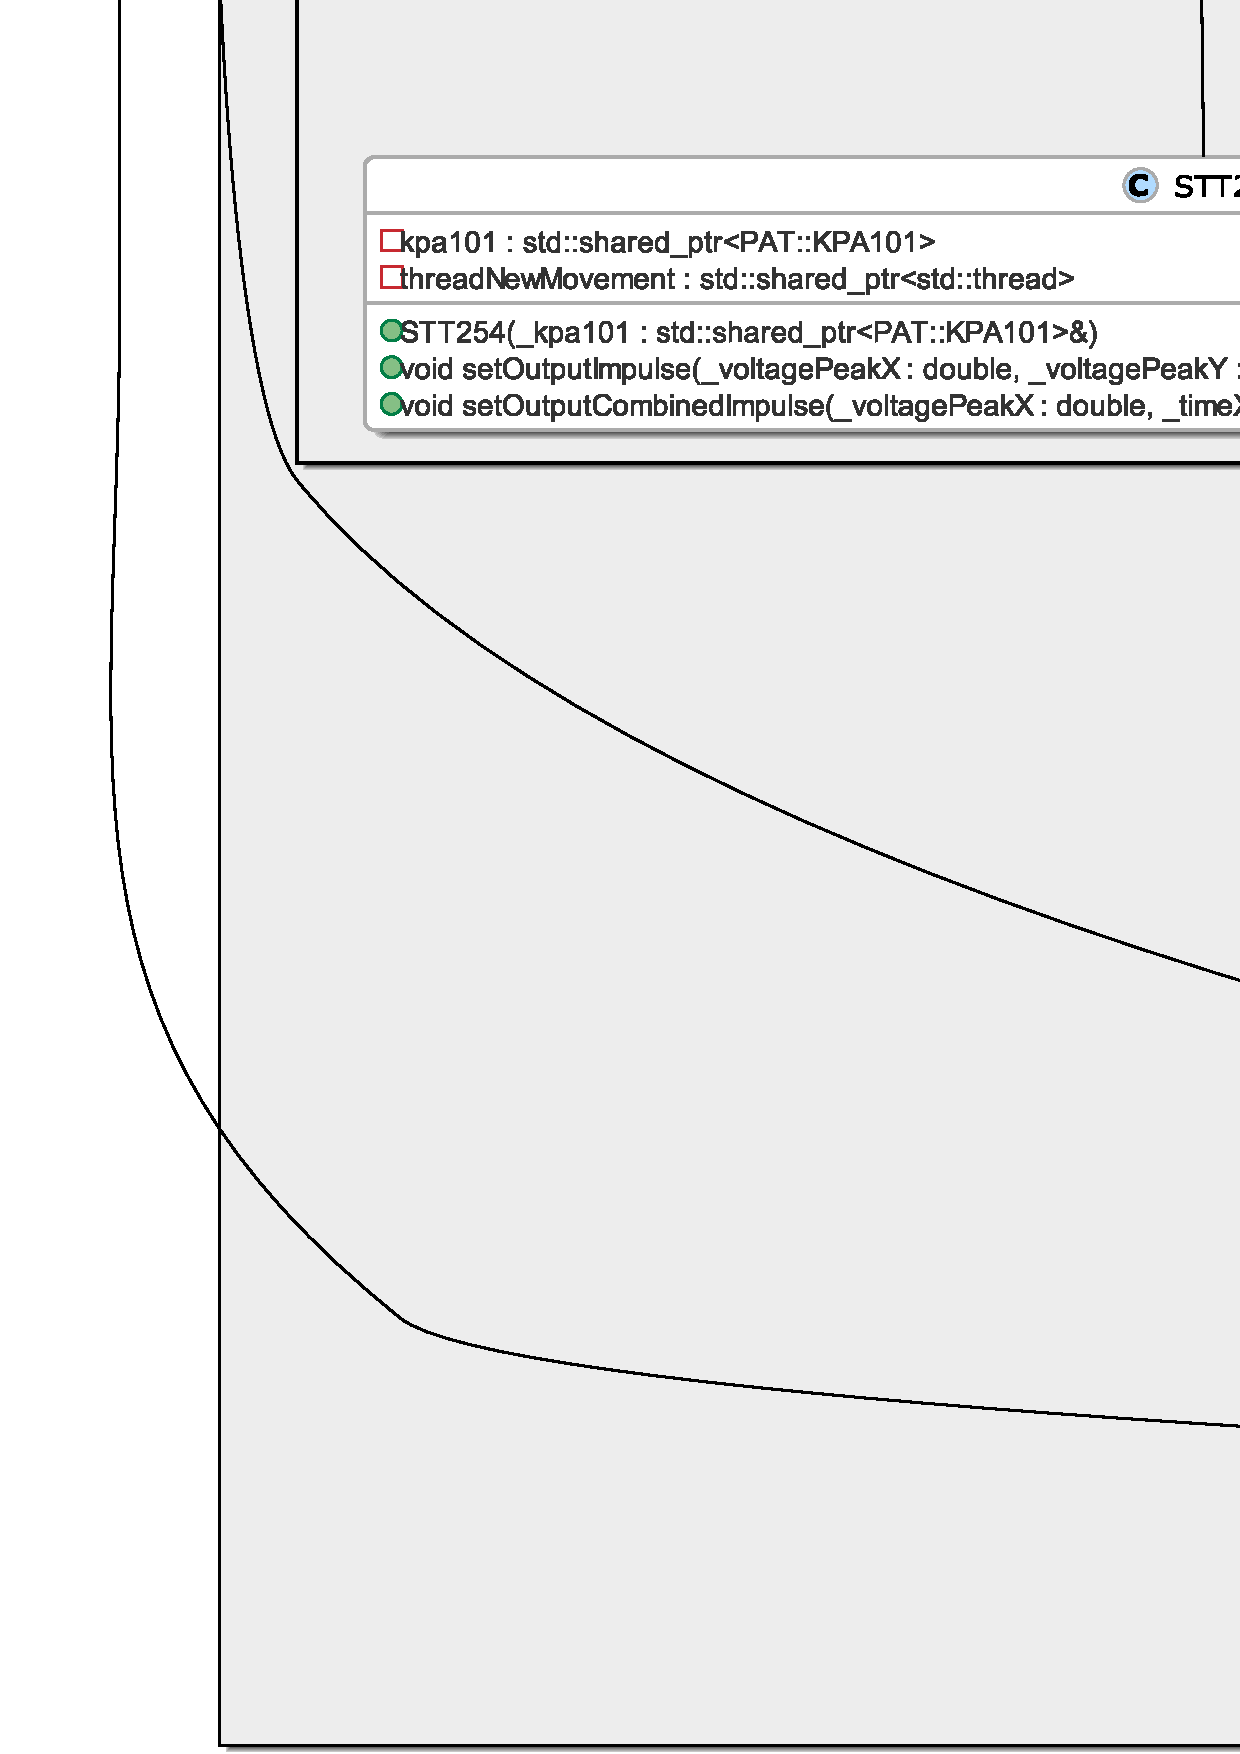
\includegraphics[width=8.33333in,height=\textheight]{https://gitlab.dei.unipd.it/pat/docs/-/raw/4da37d1e14c960824565fc73d9bca1143e667907/out/repositories/Controller/Controller.svg}
